\subsection{ASoC DAPM}

\begin{frame}{Power management with ASoC}
  \begin{itemize}
    \item Many components allow flexible routing
    \item Different routings require different components to be turned on
    \item Many combinations: code to enable only what is needed tends to be
      complex and not easy to maintain
  \end{itemize}
  \centering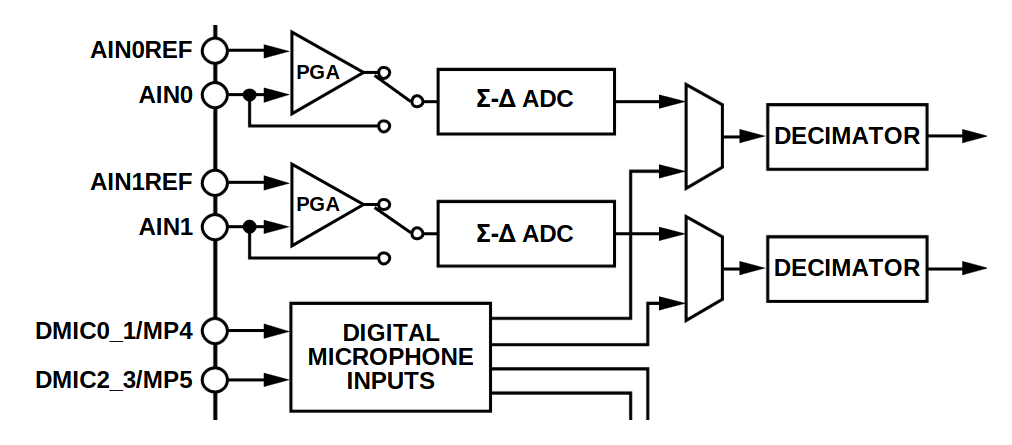
\includegraphics[height=0.4\textheight]{slides/audio-asoc-DAPM/adau1372.png}
  {\tiny (\url{https://www.analog.com/media/en/technical-documentation/data-sheets/ADAU1372.pdf})}
\end{frame}

\begin{frame}{DAPM: Dynamic Audio Power Management}
  \begin{itemize}
  \item The power management component of ASoC
  \item Linux Runtime PM works at the device level, $\rightarrow$ not suitable
  \item DAPM is independent from kernel Runtime PM, and co-existing
  \item Transparent to user space applications, saves as much power as
    possible by shutting down audio routes that are not in use.
  \item Describes every power-related element as a node of a graph
  \item Every power control is called a DAPM {\bf widget} (graph node)
  \item Every connection between widgets is called a DAPM {\bf route}
    (directed graph edge)
  \item DAPM automatically enables widgets based on active routes
  \end{itemize}
  \centering
  \includegraphics[height=0.23\textheight]{slides/audio-asoc-DAPM/dapm-widgets-ain0.pdf}
  \hfill
  \includegraphics[height=0.23\textheight]{slides/audio-asoc-DAPM/dapm-widgets-dmic0.pdf}
\end{frame}

\begin{frame}{DAPM: Dynamic Audio Power Management}
  \begin{itemize}
  \item DAPM widgets can be controlled by a regular kcontrol
  \end{itemize}
  \centering\includegraphics[height=0.35\textheight]{slides/audio-asoc-DAPM/dapm-mux.pdf}
\end{frame}

\begin{frame}{DAPM: Dynamic Audio Power Management}
  \begin{itemize}
  \item The DAPM tree spans the whole card
    \begin{itemize}
    \item In-component widgets and routes are implemented by the component
      driver
    \item Border widgets and cross-component routes are added by the card
    \end{itemize}
  \end{itemize}
  \centering\includegraphics[width=\textwidth]{slides/audio-asoc-DAPM/dapm-widgets-cross-components.pdf}
\end{frame}

\begin{frame}[t]{Endpoint widgets}
  \vspace{0.5cm}
  \centering\includegraphics[width=0.7\textwidth]{slides/audio-asoc-DAPM/widgets-endpoint.pdf}
  \vspace{1cm}
  \begin{itemize}
  \item Widgets where the sound stream originates from or terminates at
  \item ADC, DAC (PCM waveform to/from memory)
  \item Speaker, Line out, Microphone, \dots
  \end{itemize}
\end{frame}

\begin{frame}[t]{Pass-through widgets}
  \vspace{0.5cm}
  \centering\includegraphics[width=0.7\textwidth]{slides/audio-asoc-DAPM/widgets-pass-through.pdf}
  \vspace{1cm}
  \begin{itemize}
  \item Widgets on a route between other widgets
  \item Sound modifiers (PGA, Effect)
  \item Routing: Mixer, Mux, Demux, Switch
  \end{itemize}
\end{frame}

\begin{frame}[t]{Supply widgets}
  \vspace{0.5cm}
  \centering\includegraphics[width=0.7\textwidth]{slides/audio-asoc-DAPM/widgets-supply.pdf}
  \vspace{0.5cm}
  \begin{itemize}
  \item Suppliers to other widgets
  \item Clock, current, voltage
  \end{itemize}
\end{frame}

\begin{frame}[fragile]{Defining DAPM widgets}
  \begin{itemize}
  \item A widget is defined by \kstruct{snd_soc_dapm_widget}
  \end{itemize}
  \begin{block}{\kfile{include/sound/soc-dapm.h}}
    \fontsize{9}{9}\selectfont
    \begin{minted}{c}
struct snd_soc_dapm_widget {
    enum snd_soc_dapm_type id;
    const char *name;                             /* widget name */
    const char *sname;                            /* stream name */
    struct snd_soc_dapm_context *dapm;
    /* ... */
    struct pinctrl *pinctrl;                      /* attached pinctrl */
    /* ... */
    int reg;                                      /* negative reg = no direct dapm */
    unsigned char shift;                          /* bits to shift */
    unsigned int mask;                            /* non-shifted mask */
    unsigned int on_val;                          /* on state value */
    unsigned int off_val;                         /* off state value */
    /* ... */
    unsigned short event_flags;                   /* flags to specify event types */
    int (*event)(struct snd_soc_dapm_widget*, struct snd_kcontrol *, int);
};
    \end{minted}
  \end{block}
\end{frame}

\begin{frame}[fragile]{\code{snd_soc_dapm_widget}}
  \begin{itemize}
  \item An array of \kstruct{snd_soc_dapm_widget} is registered
    by the component.
  \item Many helpers exist to avoid filling the struct manually:
  \begin{block}{\kfile{include/sound/soc-dapm.h}}
    \fontsize{8}{7}\selectfont
    \begin{minted}{c}
#define SND_SOC_DAPM_INPUT(wname) \
{       .id = snd_soc_dapm_input, .name = wname, .kcontrol_news = NULL, \
        .num_kcontrols = 0, .reg = SND_SOC_NOPM }
#define SND_SOC_DAPM_OUTPUT(wname) \
{       .id = snd_soc_dapm_output, .name = wname, .kcontrol_news = NULL, \
        .num_kcontrols = 0, .reg = SND_SOC_NOPM }
#define SND_SOC_DAPM_MIC(wname, wevent) \
{       .id = snd_soc_dapm_mic, .name = wname, .kcontrol_news = NULL, \
        .num_kcontrols = 0, .reg = SND_SOC_NOPM, .event = wevent, \
        .event_flags = SND_SOC_DAPM_PRE_PMU | SND_SOC_DAPM_POST_PMD}
[...]
#define SND_SOC_DAPM_PGA(wname, wreg, wshift, winvert,\
         wcontrols, wncontrols) \
{       .id = snd_soc_dapm_pga, .name = wname, \
        SND_SOC_DAPM_INIT_REG_VAL(wreg, wshift, winvert), \
        .kcontrol_news = wcontrols, .num_kcontrols = wncontrols}
[...]
#define SND_SOC_DAPM_MUX(wname, wreg, wshift, winvert, wcontrols) \
{       .id = snd_soc_dapm_mux, .name = wname, \
        SND_SOC_DAPM_INIT_REG_VAL(wreg, wshift, winvert), \
        .kcontrol_news = wcontrols, .num_kcontrols = 1}
#define SND_SOC_DAPM_DEMUX(wname, wreg, wshift, winvert, wcontrols) \
{       .id = snd_soc_dapm_demux, .name = wname, \
        SND_SOC_DAPM_INIT_REG_VAL(wreg, wshift, winvert), \
        .kcontrol_news = wcontrols, .num_kcontrols = 1}
    \end{minted}
  \end{block}
  \end{itemize}
\end{frame}

\begin{frame}[fragile]{\code{snd_soc_dapm_widget}}
  \begin{block}{\kfile{include/sound/soc-dapm.h}}
    \fontsize{8}{7}\selectfont
    \begin{minted}{c}
#define SND_SOC_DAPM_DAC(wname, stname, wreg, wshift, winvert) \
{       .id = snd_soc_dapm_dac, .name = wname, .sname = stname, \
        SND_SOC_DAPM_INIT_REG_VAL(wreg, wshift, winvert) }
#define SND_SOC_DAPM_DAC_E(wname, stname, wreg, wshift, winvert, \
                           wevent, wflags)                                \
{       .id = snd_soc_dapm_dac, .name = wname, .sname = stname, \
        SND_SOC_DAPM_INIT_REG_VAL(wreg, wshift, winvert), \
        .event = wevent, .event_flags = wflags}

#define SND_SOC_DAPM_ADC(wname, stname, wreg, wshift, winvert) \
{       .id = snd_soc_dapm_adc, .name = wname, .sname = stname, \
        SND_SOC_DAPM_INIT_REG_VAL(wreg, wshift, winvert), }
#define SND_SOC_DAPM_ADC_E(wname, stname, wreg, wshift, winvert, \
                           wevent, wflags)                                \
{       .id = snd_soc_dapm_adc, .name = wname, .sname = stname, \
        SND_SOC_DAPM_INIT_REG_VAL(wreg, wshift, winvert), \
        .event = wevent, .event_flags = wflags}


/* generic widgets */
#define SND_SOC_DAPM_REG(wid, wname, wreg, wshift, wmask, won_val, woff_val) \
{       .id = wid, .name = wname, .kcontrol_news = NULL, .num_kcontrols = 0, \
        .reg = wreg, .shift = wshift, .mask = wmask, \
        .on_val = won_val, .off_val = woff_val, }
#define SND_SOC_DAPM_SUPPLY(wname, wreg, wshift, winvert, wevent, wflags) \
{       .id = snd_soc_dapm_supply, .name = wname, \
        SND_SOC_DAPM_INIT_REG_VAL(wreg, wshift, winvert), \
        .event = wevent, .event_flags = wflags}
#define SND_SOC_DAPM_REGULATOR_SUPPLY(wname, wdelay, wflags)            \
{       .id = snd_soc_dapm_regulator_supply, .name = wname, \
        .reg = SND_SOC_NOPM, .shift = wdelay, .event = dapm_regulator_event, \
        .event_flags = SND_SOC_DAPM_PRE_PMU | SND_SOC_DAPM_POST_PMD, \
        .on_val = wflags}
    \end{minted}
  \end{block}
\end{frame}

\begin{frame}[fragile]{DAPM example}
  \begin{block}{\kfile{sound/soc/codecs/pcm3168a.c}}
    \fontsize{8}{7}\selectfont
    \begin{minted}{c}
static const struct snd_soc_dapm_widget pcm3168a_dapm_widgets[] = {
        SND_SOC_DAPM_DAC("DAC1", "Playback", PCM3168A_DAC_OP_FLT,
                        PCM3168A_DAC_OPEDA_SHIFT, 1),
        SND_SOC_DAPM_DAC("DAC2", "Playback", PCM3168A_DAC_OP_FLT,
                        PCM3168A_DAC_OPEDA_SHIFT + 1, 1),
        SND_SOC_DAPM_DAC("DAC3", "Playback", PCM3168A_DAC_OP_FLT,
                        PCM3168A_DAC_OPEDA_SHIFT + 2, 1),
        SND_SOC_DAPM_DAC("DAC4", "Playback", PCM3168A_DAC_OP_FLT,
                        PCM3168A_DAC_OPEDA_SHIFT + 3, 1),

        SND_SOC_DAPM_OUTPUT("AOUT1L"),
        SND_SOC_DAPM_OUTPUT("AOUT1R"),
        SND_SOC_DAPM_OUTPUT("AOUT2L"),
        SND_SOC_DAPM_OUTPUT("AOUT2R"),
        SND_SOC_DAPM_OUTPUT("AOUT3L"),
        SND_SOC_DAPM_OUTPUT("AOUT3R"),
        SND_SOC_DAPM_OUTPUT("AOUT4L"),
        SND_SOC_DAPM_OUTPUT("AOUT4R"),
    \end{minted}
  \end{block}
  Note: on the \href{https://www.ti.com/lit/gpn/pcm3168a}{PCM3168A} DACs
  and ADCs can only be powered down in pairs.
\end{frame}

\begin{frame}[fragile]{DAPM example}
  \begin{block}{\kfile{sound/soc/codecs/pcm3168a.c}}
    \fontsize{8}{7}\selectfont
    \begin{minted}{c}
        SND_SOC_DAPM_ADC("ADC1", "Capture", PCM3168A_ADC_PWR_HPFB,
                        PCM3168A_ADC_PSVAD_SHIFT, 1),
        SND_SOC_DAPM_ADC("ADC2", "Capture", PCM3168A_ADC_PWR_HPFB,
                        PCM3168A_ADC_PSVAD_SHIFT + 1, 1),
        SND_SOC_DAPM_ADC("ADC3", "Capture", PCM3168A_ADC_PWR_HPFB,
                        PCM3168A_ADC_PSVAD_SHIFT + 2, 1),

        SND_SOC_DAPM_INPUT("AIN1L"),
        SND_SOC_DAPM_INPUT("AIN1R"),
        SND_SOC_DAPM_INPUT("AIN2L"),
        SND_SOC_DAPM_INPUT("AIN2R"),
        SND_SOC_DAPM_INPUT("AIN3L"),
        SND_SOC_DAPM_INPUT("AIN3R")
};
    \end{minted}
  \end{block}
\end{frame}

\begin{frame}[fragile]{\code{snd_soc_dapm_route}}
  \begin{itemize}
  \item An array of \kstruct{snd_soc_dapm_route} is registered
    by the component to define the routes.
  \end{itemize}
  \begin{block}{\kfile{include/sound/soc-dapm.h}}
    \fontsize{9}{9}\selectfont
    \begin{minted}{c}
struct snd_soc_dapm_route {
        const char *sink;
        const char *control;
        const char *source;

        /* Note: currently only supported for links where source is a supply */
        int (*connected)(struct snd_soc_dapm_widget *source,
                         struct snd_soc_dapm_widget *sink);

        struct snd_soc_dobj dobj;
};
    \end{minted}
  \end{block}
\end{frame}

\begin{frame}[fragile]{DAPM routes example}
  \begin{block}{\kfile{sound/soc/codecs/pcm3168a.c}}
    \fontsize{9}{9}\selectfont
    \begin{minted}{c}
static const char * const adau1372_decimator_mux_text[] = { "ADC", "DMIC", };
static SOC_ENUM_SINGLE_DECL(adau1372_decimator0_1_mux_enum, ADAU1372_REG_ADC_CTRL2,
                            2, adau1372_decimator_mux_text);

static const struct snd_soc_dapm_route adau1372_dapm_routes[] = {
    { "PGA0",           NULL,   "AIN0"        },
    { "ADC0",           NULL,   "PGA0"        },
    { "Decimator0 Mux", "ADC",  "ADC0"        },
    { "Decimator0 Mux", "DMIC", "DMIC0_1"     },
    { "HPOUTL",         NULL,   "OP_STAGE_LP" },
    { "HPOUTL",         NULL,   "OP_STAGE_LN" },
    /* ... */
};
    \end{minted}
  \end{block}
  \begin{itemize}
  \item Control is a standard ALSA kcontrol for selection of mux input,
    demux output, mixer levels, PGA gain, \dots
  \item Matching based on strings
  \end{itemize}
\end{frame}

\begin{frame}[fragile]{Adding DAPM widgets and routes}
  \begin{itemize}
  \item Just point to the defined arrays in
    \kstruct{snd_soc_component_driver}
  \end{itemize}
  \begin{block}{}
    \fontsize{9}{9}\selectfont
    \begin{minted}{c}
static const struct snd_soc_component_driver adau1372_driver = {
    .set_bias_level = adau1372_set_bias_level,
    .controls = adau1372_controls,
    .num_controls = ARRAY_SIZE(adau1372_controls),
    .dapm_widgets = adau1372_dapm_widgets,
    .num_dapm_widgets = ARRAY_SIZE(adau1372_dapm_widgets),
    .dapm_routes = adau1372_dapm_routes,
    .num_dapm_routes = ARRAY_SIZE(adau1372_dapm_routes),
};
    \end{minted}
  \end{block}
\end{frame}

\begin{frame}[fragile]{Adding DAPM widgets and routes dynamically}
  \begin{itemize}
  \item DAPM routes can be added dynamically, e.g. based on codec model
  \end{itemize}
  \begin{block}{}
    \fontsize{9}{9}\selectfont
    \begin{minted}{c}
static const struct snd_soc_dapm_widget wm8994_dapm_widgets[] = { ... };
static const struct snd_soc_dapm_route wm8994_intercon[] = { ... };

static int wm8994_component_probe(struct snd_soc_component *component)
{
    /* ... */
    switch (control->type) {
    case WM8994:
        snd_soc_dapm_new_controls(dapm, wm8994_specific_dapm_widgets,
                                  ARRAY_SIZE(wm8994_specific_dapm_widgets));
        /* ... */
        snd_soc_dapm_add_routes(dapm, wm8994_intercon,
                                ARRAY_SIZE(wm8994_intercon));
        /* ... */
    }
}
    \end{minted}
  \end{block}
\end{frame}

\begin{frame}[fragile]{Connecting widgets to the DAI stream}
  \begin{itemize}
  \item The endpoints of the DAPM graph are
    \begin{itemize}
    \item The external input/output pins
      \begin{itemize}
        \item \code{SND_SOC_DAPM_INPUT()}, \code{SND_SOC_DAPM_OUTPUT()}
      \end{itemize}
    \item The DAI (digital audio interface)
      \begin{itemize}
      \item Via the stream name defined by the DAI driver, using
        (sub)string-based matching
      \end{itemize}
    \end{itemize}
  \end{itemize}
  \begin{block}{}
    \fontsize{9}{9}\selectfont
    \begin{minted}{c}
static const struct snd_soc_dapm_widget wm9705_dapm_widgets[] = {
    SND_SOC_DAPM_DAC("Left DAC",  "Left HiFi Playback",  SND_SOC_NOPM, 0, 0),
    SND_SOC_DAPM_DAC("Right DAC", "Right HiFi Playback", SND_SOC_NOPM, 0, 0),

...

static struct snd_soc_dai_driver wm9705_dai[] = {
    {
        .name = "wm9705-hifi",
        .playback = {
            .stream_name = "HiFi Playback",
...
    \end{minted}
  \end{block}
\end{frame}
\begin{frame}[t]{Phase 1: determining power state}
  \vspace{0.5cm}
  \centering\includegraphics[width=0.7\textwidth]{slides/audio-asoc-DAPM/powerstate1.pdf}
  \vspace{0.5cm}
  \begin{itemize}
  \item Source widgets are powered if they are active (used by a stream)
    and have a route to an active sink widget
  \item Sink widgets are powered if they are active (used by a stream) and
    have a route to an active source widget
  \end{itemize}
\end{frame}

\begin{frame}[t]{Phase 1: determining power state}
  \vspace{0.5cm}
  \centering\includegraphics[width=0.7\textwidth]{slides/audio-asoc-DAPM/powerstate2.pdf}
  \vspace{0.5cm}
  \begin{itemize}
  \item Pass-through widgets are powered if they are on the route between two
    powered endpoint widgets
  \item Computed by DAPM automatically
  \end{itemize}
\end{frame}

\begin{frame}[t]{Phase 1: determining power state}
  \vspace{0.5cm}
  \centering\includegraphics[width=0.7\textwidth]{slides/audio-asoc-DAPM/powerstate3.pdf}
  \vspace{0.5cm}
  \begin{itemize}
  \item Supply widgets are powered if they have a path to a powered widget
  \item Computed by DAPM automatically
  \end{itemize}
\end{frame}

\begin{frame}{Phase 2: Powering sequence}
  \begin{enumerate}
  \item Compute difference between previous and new configurations
  \item Power down newly-disabled widgets
  \item Apply routing changes
  \item Power up newly-enabled widgets
  \end{enumerate}
\end{frame}

\begin{frame}[fragile]{debugfs}
  \begin{itemize}
  \item Each widget is exposed as a file in  debugfs
  \item \code{/sys/kernel/debug/asoc/${CARD}/${COMPONENT}/dapm/${WIDGET}}
  \item \code{/sys/kernel/debug/asoc/${CARD}/dapm/${WIDGET}} for card-level widgets
  \begin{block}{}
    \fontsize{9}{9}\selectfont
    \begin{minted}{shell}
# cat "/sys/kernel/debug/asoc/STM32MP15-DK/cs42l51.0-004a/dapm/Left ADC"
Left ADC: Off  in 1 out 0 - R2(0x2) mask 0x2
 stream Left HiFi Capture inactive
 widget-type adc
 out  "static" "Capture" "cs42l51.0-004a"
 in  "static" "Left PGA" "cs42l51.0-004a"
#
    \end{minted}
  \end{block}
  \item Format was improved in v6.10
  \end{itemize}
\end{frame}

\begin{frame}[fragile]{vizdapm}
  \begin{itemize}
  \item Simple shell script developed by Dimitris Papastamos, Wolfson Micro
  \item Generates a graph of DAPM widgets and routes as a PNG picture
  \item Based on \code{dot} from graphviz
  \item Repository disappeared, still available in some git forks
  \end{itemize}
  \begin{block}{}
    \fontsize{9}{9}\selectfont
    \begin{minted}{shell}
# vizdapm /sys/kernel/debug/asoc/STM32MP15-DK/cs42l51.0-004a/dapm out.png
    \end{minted}
  \end{block}
\end{frame}

\begin{frame}{vizdapm}
    \centering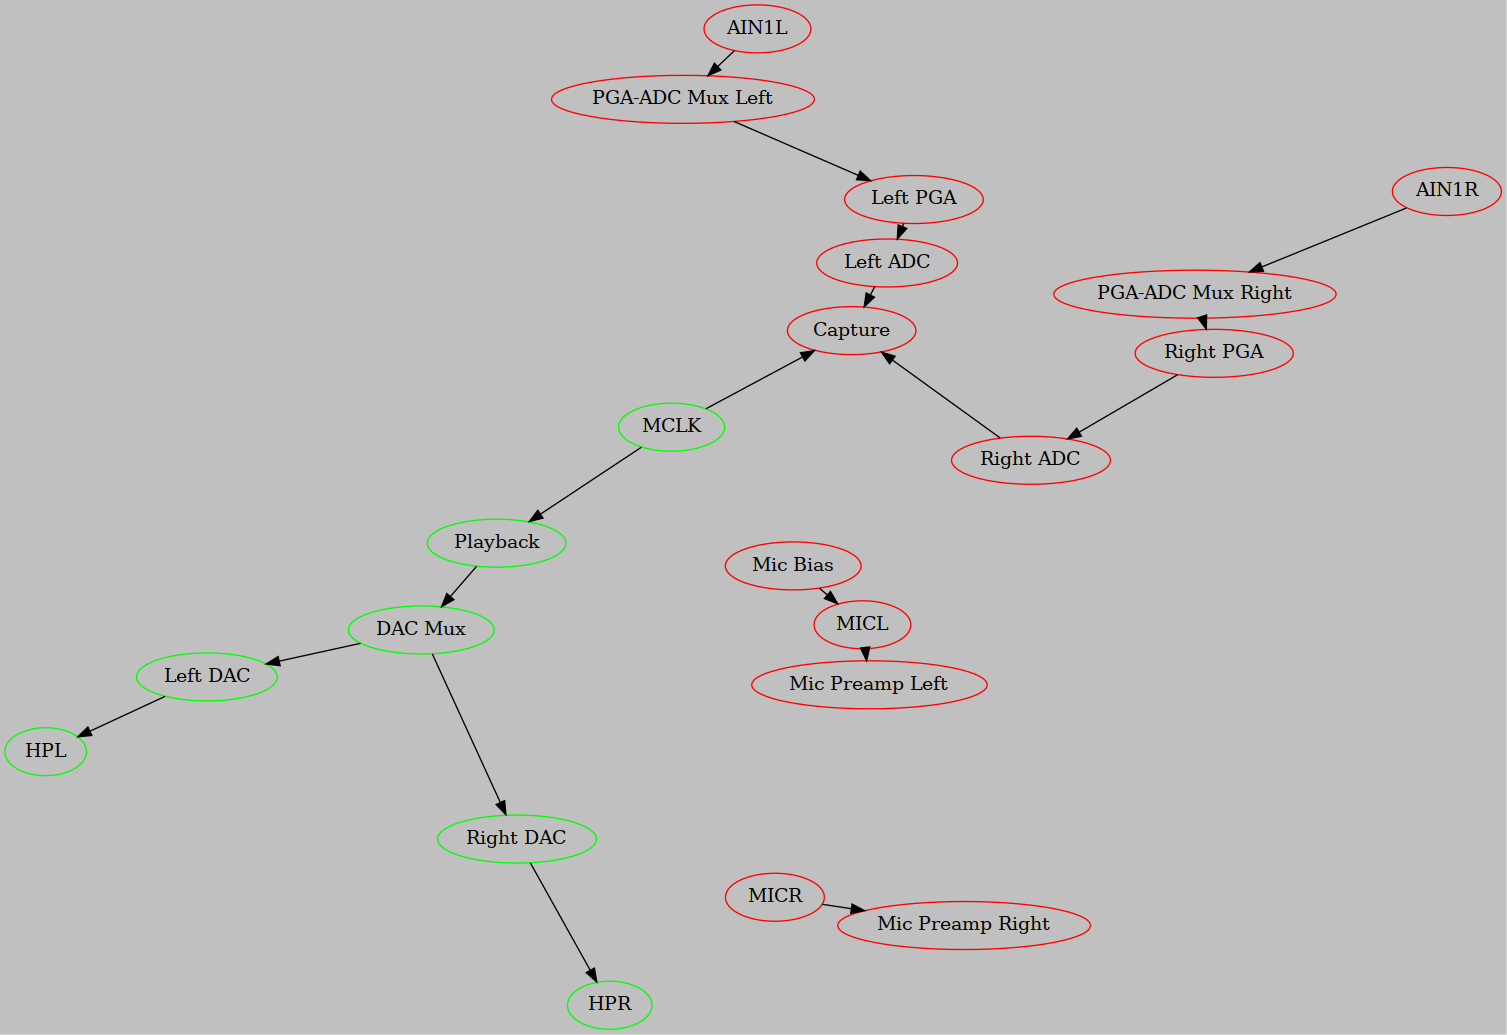
\includegraphics[height=0.8\textheight]{slides/audio-asoc-DAPM/graphviz.png}
\end{frame}

\begin{frame}{dapm-graph}
  \begin{itemize}
  \item Inspired by vizdapm and also based on \code{dot} from graphviz
  \item Yet another shell script but more powerful and simpler to use
  \item Shows all components and their connections
  \item Works with BuyBox shell
  \item Basic usage:
    \begin{itemize}
    \item \code{dapm-graph -o dapm.svg -c STM32MP15-DK}
    \end{itemize}
  \item Remote mode:
    \begin{itemize}
    \item \code{dapm-graph -o dapm.svg -c STM32MP15-DK -r root@192.168.0.1}
    \item Gets the status from target, processes on the host
    \end{itemize}
  \item And more
  \item Distributed with the kernel sources since v6.10
  \end{itemize}
\end{frame}

\begin{frame}[fragile]{dapm-graph}
  \begin{block}{}
    \fontsize{9}{9}\selectfont
    \begin{minted}{text}
Usage:
    dapm-graph [options] -c CARD                  - Local sound card
    dapm-graph [options] -c CARD -r REMOTE_TARGET - Card on remote system
    dapm-graph [options] -d STATE_DIR             - Local directory

Options:
    -c CARD             Sound card to get DAPM state of
    -r REMOTE_TARGET    Get DAPM state from REMOTE_TARGET via SSH and SCP
                        instead of using a local sound card
    -d STATE_DIR        Get DAPM state from a local copy of a debugfs tree
    -o OUT_FILE         Output file (default: dapm.dot)
    -D                  Show verbose debugging info
    -h                  Print this help and exit
    \end{minted}
  \end{block}
\end{frame}

\begin{frame}{dapm-graph}
    \centering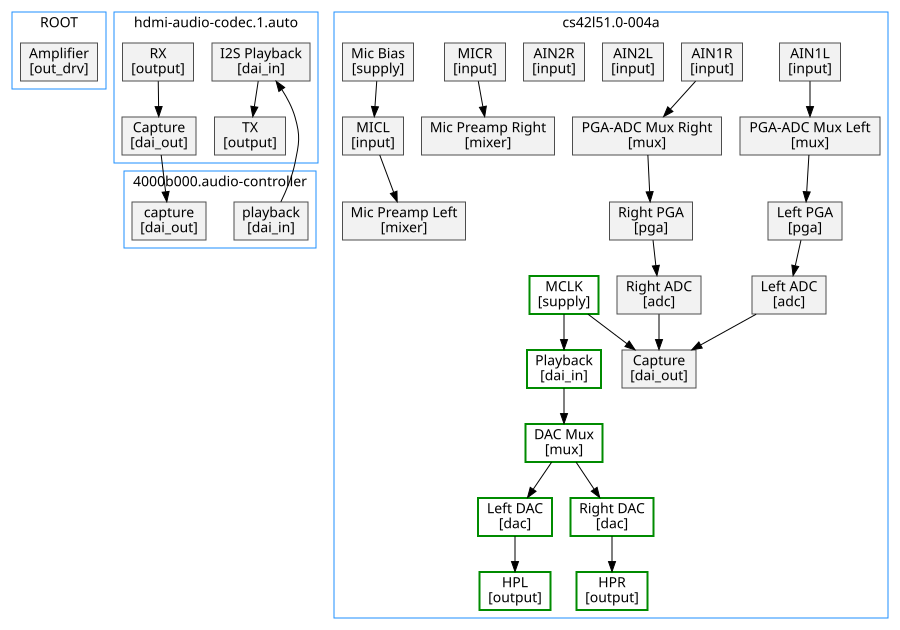
\includegraphics[height=0.8\textheight]{slides/audio-asoc-DAPM/dapm-graph.pdf}
\end{frame}


